\documentclass[11pt]{charter}

% El títulos de la memoria, se usa en la carátula y se puede usar el cualquier lugar del documento con el comando \ttitle
\titulo{Robot móvil de inspección y desinfección} 

% Nombre del posgrado, se usa en la carátula y se puede usar el cualquier lugar del documento con el comando \degreename
\posgrado{Carrera de Especialización en Sistemas Embebidos} 
%\posgrado{Carrera de Especialización en Internet de las Cosas} 
%\posgrado{Carrera de Especialización en Intelegencia Artificial}
%\posgrado{Maestría en Sistemas Embebidos} 
%\posgrado{Maestría en Internet de las cosas}

% Tu nombre, se puede usar el cualquier lugar del documento con el comando \authorname
\autor{Sergio Alberino} 

% El nombre del director y co-director, se puede usar el cualquier lugar del documento con el comando \supname y \cosupname y \pertesupname y \pertecosupname
\director{Claudio Verrastro}
\pertenenciaDirector{CNEA, UTN.BA} 
% FIXME:NO IMPLEMENTADO EL CODIRECTOR ni su pertenencia
\codirector{} % si queda vacio no se deberíá incluir 
\pertenenciaCoDirector{}

% Nombre del cliente, quien va a aprobar los resultados del proyecto, se puede usar con el comando \clientename y \empclientename
\cliente{Grupo de Inteligencia Artificial y Robótica}
\empresaCliente{Universidad Tecnológica Nacional - Facultad Regional Buenos Aires}

% Nombre y pertenencia de los jurados, se pueden usar el cualquier lugar del documento con el comando \jurunoname, \jurdosname y \jurtresname y \perteunoname, \pertedosname y \pertetresname.
\juradoUno{Nombre y Apellido (1)}
\pertenenciaJurUno{pertenencia (1)} 
\juradoDos{Nombre y Apellido (2)}
\pertenenciaJurDos{pertenencia (2)}
\juradoTres{Nombre y Apellido (3)}
\pertenenciaJurTres{pertenencia (3)}
 
\fechaINICIO{22 de junio de 2020}		%Fecha de inicio de la cursada de GdP \fechaInicioName
\fechaFINALPlanificacion{22 de Agosto de 2020} 	%Fecha de final de cursada de GdP
\fechaFINALTrabajo{22 de diciembre de 2020}		%Fecha de defensa pública del trabajo final


\begin{document}

\maketitle
\thispagestyle{empty}
\pagebreak


\thispagestyle{empty}
{\setlength{\parskip}{0pt}
\tableofcontents{}
}
\pagebreak


\section{Registros de cambios}
\label{sec:registro}


\begin{table}[ht]
\label{tab:registro}
\centering

\begin{tabularx}{\linewidth}{@{}|c|X|c|@{}}
\hline
\rowcolor[HTML]{C0C0C0} 
Revisión & \multicolumn{1}{c|}{\cellcolor[HTML]{C0C0C0}Detalles de los cambios realizados} & Fecha      \\ \hline
1.0      & Creación del documento                                                          & 27/06/2020 \\ \hline
1.1      & Cambios a partir de corrección del docente                                                                                																						   & 16/07/2020 \\ \hline
\end{tabularx}
\end{table}

\pagebreak



\section{Acta de constitución del Proyecto}
\label{sec:acta}

\begin{flushright}
Buenos Aires, \fechaInicioName
\end{flushright}

\vspace{2cm}

Por medio de la presente se acuerda con el Ing. \authorname\hspace{1px} que su Trabajo Final de la \degreename\hspace{1px} se titulará ``\ttitle'', consistirá esencialmente en el prototipo preliminar de un robot móvil útil para tareas semiautónomas de inspección y desinfección, y tendrá un presupuesto preliminar estimado de 600 hs de trabajo y \$20.000, con fecha de inicio \fechaInicioName\hspace{1px} y fecha de presentación pública \fechaFinalName.

Se adjunta a esta acta la planificación inicial.

\vfill

% Esta parte se construye sola con la información que hayan cargado en el preámbulo del documento y no debe modificarla
\begin{table}[ht]
\centering
\begin{tabular}{ccc}
\begin{tabular}[c]{@{}c@{}}Ariel Lutenberg \\ Director posgrado FIUBA\end{tabular} &  & \begin{tabular}[c]{@{}c@{}}Juan Carlos Gómz por \clientename \\ \empclientename \end{tabular} \vspace{2.5cm} \\ 
\multicolumn{3}{c}{\begin{tabular}[c]{@{}c@{}} \supname \\ Director del Trabajo Final\end{tabular}} \vspace{2.5cm} \\
\begin{tabular}[c]{@{}c@{}}\jurunoname \\ Jurado del Trabajo Final\end{tabular}     &  & \begin{tabular}[c]{@{}c@{}}\jurdosname\\ Jurado del Trabajo Final\end{tabular}  \vspace{2.5cm}  \\
\multicolumn{3}{c}{\begin{tabular}[c]{@{}c@{}} \jurtresname\\ Jurado del Trabajo Final\end{tabular}} \vspace{.5cm}                                                                     
\end{tabular}
\end{table}




\section{Descripción técnica-conceptual del Proyecto a realizar}
\label{sec:descripcion}

\begin{consigna}{black}
 La idea consiste en el desarrollo de una plataforma móvil que pueda ser controlada a distancia para inspeccionar zonas de difícil acceso o para proveer servicios de desinfección por efecto de rayos ultravioletas. Esto sería principalmente útil en instituciones médicas en las que es posible el contagio de enfermedades por la propagación de bacterias y virus en ambientes comunes.
La plataforma debería contar con una placa de procesamiento central (Edu-CIAA) que recibe datos directos (o pre-procesados por otra/s placa/s) y una placa de control para el accionamiento de motores y/o dispositivos adicionales (como puede ser el encendido de un tubo UV).
Adicionalmente, el robot podría llevar una cámara inalámbrica para dar mayor información sobre las zonas inspeccionadas. En la Figura \ref{fig:diagBloques} se presenta el diagrama en bloques del sistema. 

\vspace{25px}

\begin{figure}[htpb]
\centering 
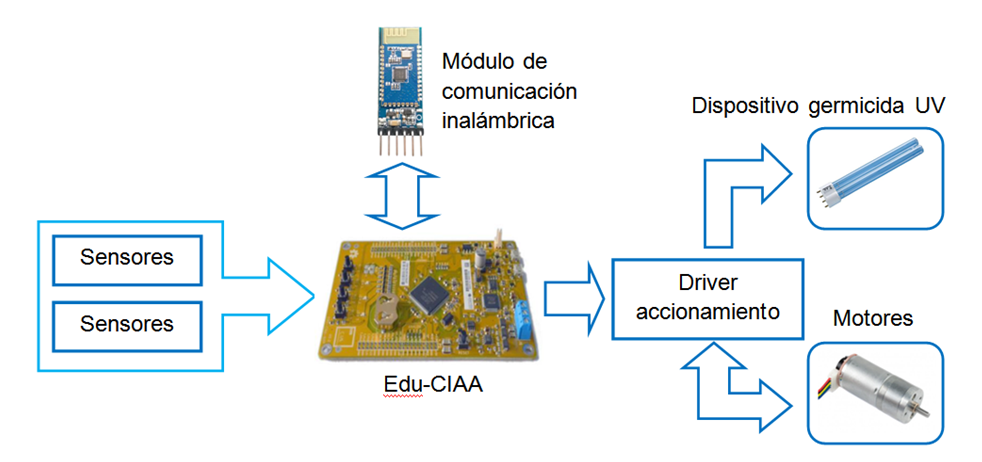
\includegraphics[width=.9\textwidth]{./Figuras/diagBloques.png}
\caption{Diagrama en bloques del sistema}
\label{fig:diagBloques}
\end{figure}

\vspace{25px}

Si bien existen plataformas robots similares, las mismas suelen estar fabricadas fuera del país, con lo que el costo de adquisición y transporte resultan particularmente elevados. Además, un desarrollo local documentado contaría con la posibilidad de soporte técnico dentro de las mismas instituciones involucradas.
La “Desinfección sin residuos químicos“ por luz ultravioleta ha demostrado efectividad como germicida, resultando letal para virus, bacterias, esporas de hongos y microorganismos superiores, ya que altera su ADN, evitando su reproducción.
Se prevé algún tipo de conectividad inalámbrica para control y obtención de datos, desde un dispositivo móvil. La idea es dejar preparada la plataforma para la posibilidad posterior de incorporación de módulos que provean servicios de valor agregado, como sensores específicos, posicionamiento GPS, etc.
La plataforma robot debe poder operar con baterías recargables que le den una autonomía aceptable para la tarea a realizar.
La presente propuesta espera ser aprovechada en el Grupo de Inteligencia Artificial y Robótica de la UTN - Facultad Regional Buenos Aires, El hardware resultante podrá ser utilizado también para la evaluación de algoritmos de Inteligencia Artificial, para aplicaciones en la industria local, y para actividades de docencia e investigación.

\end{consigna}


\section{Identificación y análisis de los interesados}
\label{sec:interesados}

\begin{consigna}{red} 

\begin{table}[ht]
%\caption{Identificación de los interesados}
%\label{tab:interesados}
\begin{tabularx}{\linewidth}{@{}|l|X|X|l|@{}}
\hline
\rowcolor[HTML]{C0C0C0} 
Rol           & Nombre y Apellido & Organización 	& Puesto 	\\ \hline
Auspiciante   &                   &              	&        	\\ \hline
Cliente       & \clientename      &\empclientename	&        	\\ \hline
Impulsor      & Secretaría de Ciencia, Tecnología e innovación productiva                  &\empclientename&        	\\ \hline
Responsable   & \authorname       & FIUBA        	& Alumno 	\\ \hline
Colaboradores &                   &              	&        	\\ \hline
Orientador    & \supname	      & \pertesupname 	& Director	Trabajo final \\ \hline
Usuario final & Personal de salud & Establecimientos hospitalarios 	&        	\\ \hline
\end{tabularx}
\end{table}


\end{consigna}



\section{1. Propósito del proyecto}
\label{sec:proposito}

\begin{consigna}{black}
El propósito de este proyecto es desarrollar un prototipo de plataforma móvil de observación para tareas semiautónomas de inspección y desinfección, con documentación completa para su reproducción a escala industrial. El dispositivo deberá poder controlarse a distancia para inspeccionar zonas de difícil acceso o para proveer servicios de desinfección por efecto de rayos ultravioletas. Esto sería principalmente útil en instituciones médicas en las que es posible el contagio de enfermedades por la propagación de bacterias y virus en ambientes comunes.
\end{consigna}

\section{2. Alcance del proyecto}\label{sec:alcance}
\begin{consigna}{black}
\vspace{-12mm}
\begin{itemize}
\item Diseño e implementación de una plataforma robot de dimensiones reducidas, con conectividad inalámbrica
\item Programación del firmware los módulos correspondientes. 
\item Programación del software de comunicaciones. 
\item Pruebas de funcionamiento.
\item Documentación del trabajo. 
\end{itemize}
El presente proyecto NO incluye: 
\begin{itemize}
\item La instalación y puesta en marcha del sistema completo de inspección y desinfección, en institución hospitalario (salvo que el tiempo disponible lo permita). 
\item El robot no monitoreará,  ni  realizará la carga de la batería.
\item No se incluye cargador.
\end{itemize}
\end{consigna}

\section{3. Supuestos del proyecto}
\label{sec:supuestos}

\begin{consigna}{black}
Para el desarrollo del presente proyecto se supone que: 

\begin{itemize}
\item Se contará con disponibilidad de los laboratorios e instrumental de la  Secretaría de Ciencia, Tecnología e innovación productiva. UTN. Buenos Aires, para cubrir la tarea de desarrollo.
\item Se dispondrá de tiempo durante la jornada laboral para la realización del mismo. 
\item  Se dispondrá de todos los componentes y herramientas necesarios. 
\end{itemize}

\end{consigna}

\section{4. Requerimientos}
\label{sec:requerimientos}
\begin{consigna}{black}
\vspace{-12mm}
\begin{enumerate}
\item Requerimientos funcionales
	\begin{enumerate}
	\item Capacidad de locomoción.  El robot debe ser capaz de desplazarse por medio de ruedas motorizadas, a través de superficies planas.
	\item Capacidad de percepción. El robot debe ser capaz de detectar y obtener información del medio. 
	\item Capacidad de comunicación inalámbrica.
	\item El robot deberá funcionar con alimentación a batería recargable.
	\item El proyecto debe ser extensible a una posible herramienta de enseñanza e investigación

	\end{enumerate}
\item Requerimientos no funcionales
	\begin{enumerate}
	\item El robot no debe resultar peligroso para el ambiente o las personas con las que podría interactuar.
	\item El diseño del robot debe respetar regulaciones en cuanto a radiación en el espectro ultravioleta.
	\item Se utilizarán componentes electrónicos disponibles comercialmente en Argentina.
	\end{enumerate}
\end{enumerate}
\end{consigna}

\section{Historias de usuarios (\textit{Product backlog})}
\label{sec:backlog}
\begin{consigna}{black}
Para las siguientes historias de usuario se tomará como criterio de ponderación el esfuerzo para lograr hacer posible la misma.\\
La prioridad se toma como orden de necesidad/utilidad del objetivo. 
La Ponderación se indica con un valor 1 a 5, siendo el valor 1 el correspondiente a la mayor esfuerzo y 5 al menor.
La Prioridad se cuantifica de 1 a 5, siendo el valor 1 el correspondiente a la mayor prioridad y 5 a la menor.

Historias de usuario Nº1: Como personal hospitalario, quiero poder hacer que el robot sanitizante se desplace a una posición específica. 
\begin{itemize}
\item Ponderación: 1 (siete)
\item Prioridad: 2 (siete)
\end{itemize}  

Historias de usuario Nº2: Como técnico del producto, quiero poder modificar parámetros de funcionamiento del robot.
\begin{itemize}
\item Ponderación: 1 (siete)
\item Prioridad: 4 (siete)
\end{itemize}  

Historias de usuario Nº3: Como personal hospitalario, quiero poder realizar la sanitización desde una distancia de aproximadamente diez metros.
\begin{itemize}
\item Ponderación: 1 (siete)
\item Prioridad: 2 (siete)
\end{itemize}  

Historias de usuario Nº4: Como personal hospitalario, quiero contar un un manual de uso detallado para saber cómo operarlo. correctamente
\begin{itemize}
\item Ponderación: 4 (siete)
\item Prioridad: 2 (siete)
\end{itemize}  

Historias de usuario Nº5: Como administrador hospitalario, quiero que el uso del robot sanitizante no resulte peligroso para ninguna persona que interactue con el mismo.
\begin{itemize}
\item Ponderación: 3 (siete)
\item Prioridad: 1 (siete)
\end{itemize}  

Historias de usuario Nº6: Como técnico del producto, quiero que el robot genere un reporte con datos de funcionamiento, para poder realizar tareas de verificación y mantenimiento.
\begin{itemize}
\item Ponderación: 2 (siete)
\item Prioridad: 3 (siete)
\end{itemize}  

\end{consigna}


\section{5. Entregables principales del proyecto}
\label{sec:entregables}
\vspace{-12mm}
\begin{consigna}{black}
\begin{itemize}
\item Prototipo funcional
\item Manual de uso
\item Diagrama esquemático del hardware
\item Códigos fuentes software
\item Informe final

\end{itemize}
\end{consigna}
\pagebreak


\section{6. Desglose del trabajo en tareas}
\label{sec:wbs}
\begin{consigna}{black}
\vspace{-12mm}
\begin{enumerate}
\item Planificación(50hs) 
	\begin{enumerate}
	\item Relevamiento de necesidades(10hs) 
	\item Análisis de requerimientos(20hs) 
	\item Confección de la planificación del proyecto(20hs) 
	\end{enumerate}
\item Diseño e implementación(155hs) 
	\begin{enumerate}
	\item Selección de materiales y componentes (10hs)
	\item Diseño de esquemáticos (35hs) 
	\item Construcción de hardware de control (35hs)
	\item Construcción de hardware de sensores (30hs)
	\item Integración de hardware (20hs)
	\item Pruebas funcionales (25hs) 
	\end{enumerate}
	\item Programación de Firmware (130hs) 
	\begin{enumerate}
	\item Programación software de control de motores  (20hs)
	\item Implementación de drivers para adquisición de datos de los sensores (20hs)
	\item Pruebas de funcionamiento (15hs)
	\item Programación de firmware de control reactivo para funcionamiento del robot (40hs) 
	\item Programación software de control comunicación(35hs) 
	\item Modificaciones para integración al software(10hs) 
	\end{enumerate}
	\item Construcción del prototipo (105hs) 
	\begin{enumerate}
	\item Diseño mecánico de la plataforma (20hs)
	\item Armado del prototipo(40hs)
	\item Pruebas funcionales de integración mecánica-electrónica (25hs)
	\item Ajuste de parámetros de funcionamiento (20hs)
	\end{enumerate}
	\item Programación de software de aplicación (85hs) 
	\begin{enumerate}
	\item Diseño de la interfaz de control (20hs) 
	\item Programación de la interfaz de control (40hs)
	\item  Pruebas y ajuste de la interfaz de control (25hs)
	\end{enumerate}
	\item Documentación y presentación (95hs) 
	\begin{enumerate}
	\item Informe de avances (10hs)
	\item Documentación del trabajo realizado (15hs) 
	\item Creación de manuales de uso (15hs) 
	\item Realización de Informe del proyecto (35hs) 
	\item Presentación final (20hs)
	\end{enumerate}
\end{enumerate}

Cantidad total de horas: (630 hs)

\end{consigna}
\pagebreak

\section{7. Diagrama de Activity On Node}
\label{sec:AoN}

\begin{consigna}{red}

\begin{figure}[htpb]
\centering 
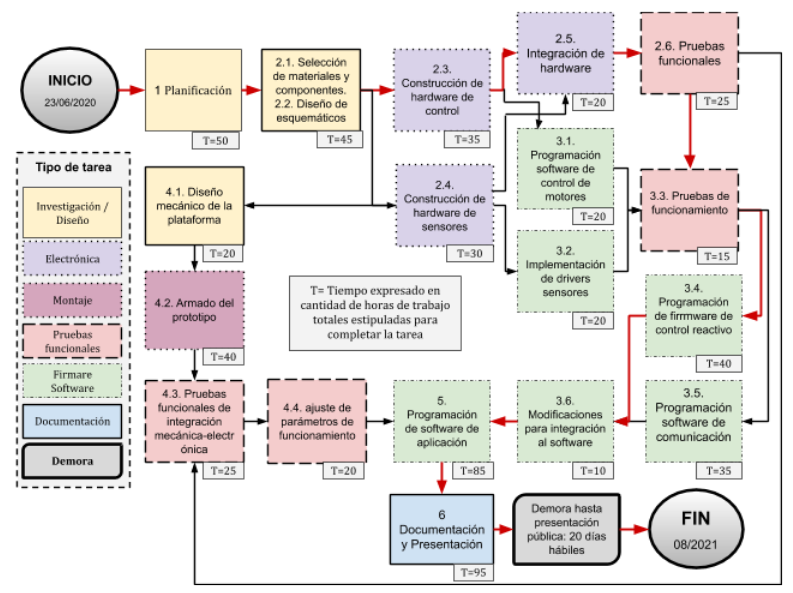
\includegraphics[width=.8\textwidth]{./Figuras/AoN.png}
\caption{Diagrama en \textit{Activity on Node}}
\label{fig:AoN}
\end{figure}

\end{consigna}
\pagebreak

\section{8. Diagrama de Gantt}
\label{sec:gantt}

\begin{consigna}{black}

\begin{figure}[htpb]
\centering 
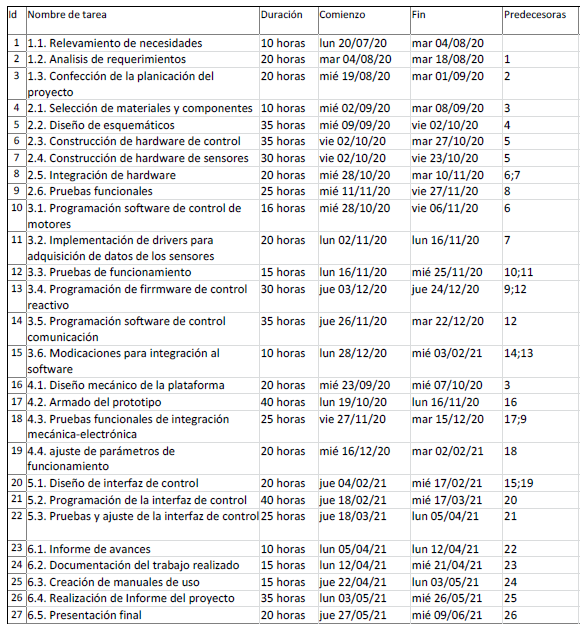
\includegraphics[width=\textwidth]{./Figuras/gantttabla.PNG}
\caption{Tabla de tareas de Gantt}
\label{fig:gantt}
\end{figure}

\begin{figure}[htpb]
\centering 
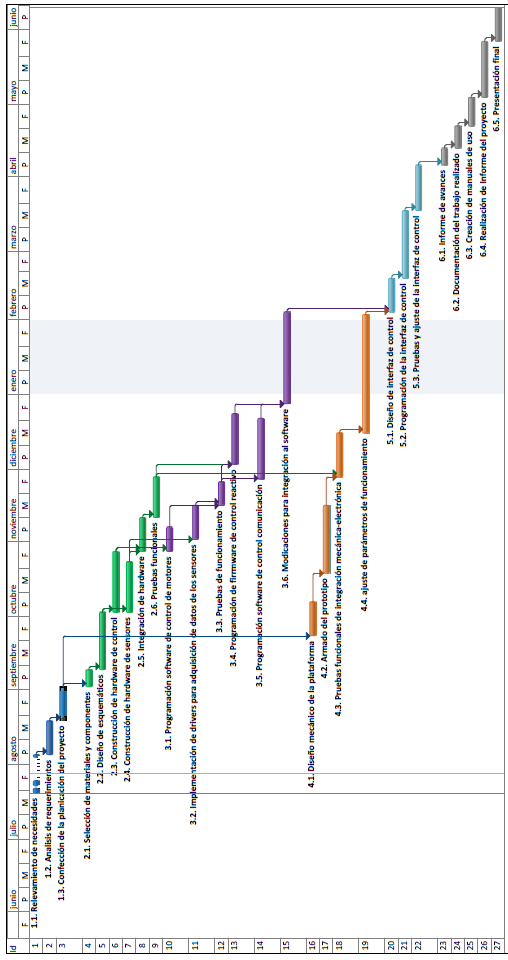
\includegraphics[width=.8\textwidth]{./Figuras/Gantt.PNG}
\caption{Diagrama de Gantt}
\label{fig:gantt}
\end{figure}
\end{consigna}
\pagebreak

\section{9. Matriz de uso de recursos de materiales}
\label{sec:recursos}

\begin{table}[htpb]
\label{tab:recursos}
\centering
%\resizebox{.9\textwidth}{!}{
\begin{tabularx}{\textwidth}{@{}|c|p{12em}|p{5em}|p{4.5em}|p{4.5em}|X|@{}}
\hline
\cellcolor[HTML]{C0C0C0} & \cellcolor[HTML]{C0C0C0} & \multicolumn{4}{c|}{\cellcolor[HTML]{C0C0C0}Recursos requeridos (horas)} \\ \cline{3-6} 
\multirow{-2}{*}{\cellcolor[HTML]{C0C0C0}\begin{tabular}[c]{@{}c@{}}Código\\ WBS\end{tabular}} 
& 
\multirow{-2}{*}{\cellcolor[HTML]{C0C0C0}\begin{tabular}[]{@{}c@{}}Nombre\\tarea\end{tabular}}
\centering
&  
PC con acceso a Internet & Placa de desarrollo & Taller de electrónica & Equipamiento mecánico / 3D \\ \hline
1 & Planificación & \multicolumn{1}{c|}{50hs}  &  &  &  \\ \hline
2.1 & Selección de materiales & \multicolumn{1}{c|}{10hs}  &  &  &  \\ \hline
2.2 & Diseño de esquemáticos & \multicolumn{1}{c|}{35hs}  &  &  &  \\ \hline
2.3 & Construcción de hardware de control & & & \multicolumn{1}{c|}{35hs} &    \\ \hline
2.4 & Construcción de hardware de sensores & & & \multicolumn{1}{c|}{30hs} &   \\ \hline
2.5 & Integración de hardware  &  &  & \multicolumn{1}{c|}{20hs} &  \\ \hline
2.6  & Pruebas funcionales    &  &  & \multicolumn{1}{c|}{25hs} &  \\ \hline
3.1 & Programación software de control de motores    &  \multicolumn{1}{c|}{20hs}  &  &  &  \\ \hline
3.2  & Implementación de drivers para sensores      & \multicolumn{1}{c|}{20hs} &  &  &  \\ \hline
3.3 & Pruebas de funcionamiento  &  & \multicolumn{1}{c|}{15hs} & \multicolumn{1}{c|}{15hs}  &  \\ \hline
3.4 & Programación de firmware de control reactivo del robot  & \multicolumn{1}{c|}{40hs}  & \multicolumn{1}{c|}{40hs} &  &  \\ \hline
3.5 & Programación software de control comunicación & \multicolumn{1}{c|}{35hs} &  &  &  \\ \hline
3.6 & Modificaciones para integración al software   & \multicolumn{1}{c|}{10hs} & \multicolumn{1}{c|}{10hs} &  &  \\ \hline   
4 & Construcción del prototipo & \multicolumn{1}{c|}{20hs} &  &  & \multicolumn{1}{c|}{85hs} \\ \hline
5.1 & Diseño de interfaz de control  & \multicolumn{1}{c|}{20hs} &  &  &  \\ \hline
5.2 &  Programación de la interfaz de control & \multicolumn{1}{c|}{20hs} & \multicolumn{1}{c|}{20hs} &  &  \\ \hline
5.3 & Pruebas y ajuste de la interfaz de control & \multicolumn{1}{c|}{25hs} & \multicolumn{1}{c|}{25hs} &  &  \\ \hline
6 & Documentación y Presentación & \multicolumn{1}{c|}{95hs} &  &  &  \\ \hline
\end{tabularx}%
\end{table}

\pagebreak

\section{10. Presupuesto detallado del proyecto}
\label{sec:presupuesto}

\begin{consigna}{black}

\vspace{-12mm}
\begin{table}[htpb]
\centering
\begin{tabularx}{\linewidth}{@{}|X|c|r|r|@{}}
\hline
\rowcolor[HTML]{C0C0C0} 
\multicolumn{4}{|c|}{\cellcolor[HTML]{C0C0C0}COSTOS DIRECTOS} \\ \hline
\rowcolor[HTML]{C0C0C0} 
Descripción &
  \multicolumn{1}{c|}{\cellcolor[HTML]{C0C0C0}Cantidad} &
  \multicolumn{1}{c|}{\cellcolor[HTML]{C0C0C0}Valor unitario} &
  \multicolumn{1}{c|}{\cellcolor[HTML]{C0C0C0}Valor total} \\ \hline
\multicolumn{1}{|l|}{ Placa Edu-CIAA} &
  \multicolumn{1}{c|}{1} &
  \multicolumn{1}{c|}{5100} &
  \multicolumn{1}{c|}{5100} \\ \hline
\multicolumn{1}{|l|}{Motor DC con reducción + Encoder} &
  \multicolumn{1}{c|}{2} &
  \multicolumn{1}{c|}{1500} &
  \multicolumn{1}{c|}{3000} \\ \hline
\multicolumn{1}{|l|}{Barra Led UvC Germicida 280nm} &
  \multicolumn{1}{c|}{1} &
  \multicolumn{1}{c|}{4000} &
  \multicolumn{1}{c|}{4000} \\ \hline
\multicolumn{1}{|l|}{Módulo Bluetooth HC-05} &
  \multicolumn{1}{c|}{1} &
  \multicolumn{1}{c|}{750} &
  \multicolumn{1}{c|}{750} \\ \hline
\multicolumn{1}{|l|}{Sensor de Distancia IR Sharp 10 A 80 Cm} &
  \multicolumn{1}{c|}{1} &
  \multicolumn{1}{c|}{1160} &
  \multicolumn{1}{c|}{1160} \\ \hline
\multicolumn{1}{|l|}{Componentes electrónicos varios} &
  \multicolumn{1}{c|}{1} &
  \multicolumn{1}{c|}{1000} &
  \multicolumn{1}{c|}{1000} \\ \hline
\multicolumn{1}{|l|}{Celda Batería Ion Litio 18650} &
  \multicolumn{1}{c|}{3} &
  \multicolumn{1}{c|}{600} &
  \multicolumn{1}{c|}{1800} \\ \hline
\multicolumn{1}{|l|}{Porta Bateria Holder 18650 X3} &
  \multicolumn{1}{c|}{1} &
  \multicolumn{1}{c|}{490} &
  \multicolumn{1}{c|}{490} \\ \hline
\multicolumn{1}{|l|}{Interruptor final de carrera} &
  \multicolumn{1}{c|}{3} &
  \multicolumn{1}{c|}{200} &
  \multicolumn{1}{c|}{600} \\ \hline
\multicolumn{1}{|l|}{sensores IR reflectivos } &
  \multicolumn{1}{c|}{1} &
  \multicolumn{1}{c|}{400} &
  \multicolumn{1}{c|}{400} \\ \hline
\multicolumn{1}{|l|}{Conectores y cables varios} &
  \multicolumn{1}{c|}{1} &
  \multicolumn{1}{c|}{500} &
  \multicolumn{1}{c|}{500} \\ \hline
\multicolumn{1}{|l|}{Materiales gabinete prototipo / PLA imp.3D} &
  \multicolumn{1}{c|}{1} &
  \multicolumn{1}{c|}{1000} &
  \multicolumn{1}{c|}{1000} \\ \hline
\multicolumn{3}{|c|}{SUBTOTAL} &
  \multicolumn{1}{c|}{19400} \\ \hline
\rowcolor[HTML]{C0C0C0} 
\multicolumn{4}{|c|}{\cellcolor[HTML]{C0C0C0}COSTOS INDIRECTOS} \\ \hline
\rowcolor[HTML]{C0C0C0} 
Descripción &
  \multicolumn{1}{c|}{\cellcolor[HTML]{C0C0C0}Cantidad} &
  \multicolumn{1}{c|}{\cellcolor[HTML]{C0C0C0}Valor unitario} &
  \multicolumn{1}{c|}{\cellcolor[HTML]{C0C0C0}Valor total} \\ \hline
\multicolumn{1}{|l|}{Se supone 20 por ciento del Costo fijo} &
  \multicolumn{1}{c|}{1} &
  \multicolumn{1}{c|}{3880} &
  \multicolumn{1}{c|}{3880} \\ \hline


\multicolumn{3}{|c|}{SUBTOTAL} &
  \multicolumn{1}{c|}{3880} \\ \hline
\rowcolor[HTML]{C0C0C0}
\multicolumn{3}{|c|}{TOTAL} &
  \multicolumn{1}{c|}{23280} 
   \\ \hline
\end{tabularx}%
\end{table}
Cotización dólar estadounidenses al 27/07/2020: oficial 72 pesos / blue 120 pesos
\end{consigna}

\section{11. Matriz de asignación de responsabilidades}
\label{sec:responsabilidades}
\begin{consigna}{black}
\vspace{-12mm}
\begin{table}[htbp]
\centering
%\resizebox{.9\textwidth}{!}{
\begin{tabularx}{\textwidth}{@{}|c|p{14em}|p{6em}|p{4.6em}|p{3em}|X|@{}}
\hline
\rowcolor[HTML]{C0C0C0} 
\cellcolor[HTML]{C0C0C0} &
  \cellcolor[HTML]{C0C0C0} &
  \multicolumn{4}{c|}{\cellcolor[HTML]{C0C0C0}Roles del proyecto} \\ \cline{3-6} 
\rowcolor[HTML]{C0C0C0} 
\cellcolor[HTML]{C0C0C0} &
  \cellcolor[HTML]{C0C0C0} &
  Responsable &
  Orientador &
  Cliente &
  Jurado \\ \cline{3-6} 
\rowcolor[HTML]{C0C0C0} 
\multirow{-3}{*}{\cellcolor[HTML]{C0C0C0}\begin{tabular}[c]{@{}c@{}}Código\\ WBS\end{tabular}} &
  \multirow{-3}{*}{\cellcolor[HTML]{C0C0C0}Nombre de la tarea} &
  \authorname &
  \supname &
  GIAR &
   \\ \hline
1 & Planificación & \multicolumn{1}{c|}{P}  & \multicolumn{1}{c|}{C} &  \multicolumn{1}{c|}{A} &  \multicolumn{1}{c|}{I} \\ \hline
2 & Diseño e implementación & \multicolumn{1}{c|}{P}  &  \multicolumn{1}{c|}{C} &  &  \\ \hline
3 & Programación Firmware    &  \multicolumn{1}{c|}{P}  &  \multicolumn{1}{c|}{C} &  &  \\ \hline
4 & Construcción del prototipo & \multicolumn{1}{c|}{P} &  &  & \\ \hline
5 & Programación software de aplicación & \multicolumn{1}{c|}{P} &  &  &  \\ \hline
6.1 &  Informe de avances & \multicolumn{1}{c|}{P} &  \multicolumn{1}{c|}{C}  & \multicolumn{1}{c|}{I} &  \\ \hline
6.2 &  Documentación del trabajo realizado & \multicolumn{1}{c|}{P} &  \multicolumn{1}{c|}{C}  & \multicolumn{1}{c|}{I} &  \\ \hline
6.3 &  Creación de manuales de uso & \multicolumn{1}{c|}{P} & \multicolumn{1}{c|}{I} &  &  \\ \hline
6.4 & Realización de Informe del proyecto & \multicolumn{1}{c|}{P} &  \multicolumn{1}{c|}{C}  & \multicolumn{1}{c|}{I} & \multicolumn{1}{c|}{I}  \\ \hline
6.5 &  Presentación final & \multicolumn{1}{c|}{P} & \multicolumn{1}{c|}{I}  & \multicolumn{1}{c|}{I} & \multicolumn{1}{c|}{A} \\ \hline

\end{tabularx}%
\end{table}


{\footnotesize
Referencias:
\begin{itemize}
	\item P = Responsabilidad Primaria
	\item S = Responsabilidad Secundaria
	\item A = Aprobación
	\item I = Informado
	\item C = Consultado
\end{itemize}
} %footnotesize
\end{consigna}


\section{12. Gestión de riesgos}
\label{sec:riesgos}

\begin{consigna}{black}
A continuación se describirán los riesgos asociados al proyecto y un plan de mitigación de los mismos, con
la finalidad de reducir la probabilidad de ocurrencia o minimizar el impacto de los mismos.
Tanto la severidad como la probabilidad de ocurrencia se indican con un valor entre 1 y 10, siendo 10 el de mayor severidad/ocurrencia 
 
Riesgo 1: Deterioro de la placa de desarrollo y prototipo.

\begin{itemize}
\item Severidad (S): 9 (nueve).\\
La Severidad en este caso es alta ya que esta situación haría imposible realizar cualquier tipo de avance práctico.
\item Probabilidad de Ocurrencia (O): 3 (tres).\\
La probabilidad de Ocurrencia baja, ya que la placa y el prototipo se encuentran en el domicilio del desarrollador. 
\end{itemize}   

Riesgo 2: : Imposibilidad de cumplir con los plazos planteados para el desarrollo del proyecto.
\begin{itemize}
\item Severidad (S):  7 (siete).\\
La Severidad es bastante alta, ya que de no lograr avanzar en el proyecto según los tiempos estimados,resultaría imposible completar el mismo en la fecha límite.
\item Ocurrencia (O): 6 (seis).\\
La Ocurrencia indicada es media, ya que no se poseen al momento de la planificación todos los conocimientos relacionados con las tareas a desarrollar.
\end{itemize}

Riesgo 3: : Retraso en tiempo de fabricación de placas electrónicas
\begin{itemize}
\item Severidad (S):  8 (ocho).\\
La severidad es elevada ya que la placas condicionan el tiempo de pruebas del software sobre las mismas.
\item Ocurrencia (O): 4 (cuatro).\\
La probabilidad de Ocurrencia resulta baja, ya que las placas no son de alta complejidad y deberían poder realizarse sin problemas.
\end{itemize}

Riesgo 4: Dificultad o demora para conseguir algunos componentes del prototipo.
\begin{itemize}
\item Severidad (S): 8 (ocho).
Severidad alta, porque la falta de algún componente del prototipo hace peligarar su construcción y puesta en marcha en el tiempo estipulado.
\item Ocurrencia (O): 5 (cinco).
La probabilidad de ocurrencia es media, ya que a pesar de haberse realizado la selección de materiales del proyecto teniendo en cuenta disponibilidad y cuestiones económicas, las mismas varían constantemente en el mercado local. 
\end{itemize}

Riesgo 5: Daño de la computadora que se usa para programar y documentar el proyecto
\begin{itemize}
\item Severidad (S): 8 (ocho).
La severidad es alta porque tanto la redacción de documentación como la programación de software se realiza con la computadora principal.
\item Ocurrencia (O): 4 (cuatro)
La probabilidad de ocurrencia no es muy alta ya que si bien la máquina no es nueva, supera con éxito chequeos periódicos.
\end{itemize}

b) Tabla de gestión de riesgos:      (El RPN se calcula como RPN=SxO)

\begin{table}[htpb]
\centering
\begin{tabularx}{\linewidth}{@{}|X|c|c|c|c|c|c|@{}}
\hline
\rowcolor[HTML]{C0C0C0} 
Riesgo & S & O & RPN & S* & O* & RPN* \\ \hline
Deterioro de la placa de desarrollo y prototipo    &  9 & 3  & \cellcolor{green}27    &    &    &      \\ \hline
Imposibilidad de cumplir con los plazos planteados para el desarrollo del proyecto   & 7  & 6  & \cellcolor{red}42    & 4  & 4   & \cellcolor{green}16     \\ \hline
Retraso en tiempo de fabricación de placas electrónicas       & 8 & 4  & \cellcolor{green} 32    &    &    &      \\ \hline
Dificultad o demora para conseguir algunos componentes del prototipo. & 8 & 5 & \cellcolor{red}40   & 5 & 3   & \cellcolor{green}15      \\ \hline
Daño de la computadora que se usa para programar y documentar el proyecto & 8  & 4  &    \cellcolor{green} 32 &    &    &      \\ \hline
\end{tabularx}%
\end{table}

Criterio adoptado: 
Se tomarán medidas de mitigación en los riesgos cuyos números de RPN sean mayores o iguales a 40.

Nota: los valores marcados con (*) en la tabla corresponden luego de haber aplicado la mitigación.

c) Plan de mitigación de los riesgos que originalmente excedían el RPN máximo establecido:
 
Riesgo 2: Imposibilidad de cumplir con los plazos planteados para el desarrollo del proyecto.\\
Medidas de mitigación: Consultar a  profesionales que dominen los temas que llevan a no poder cumplir con los plazos. Reestructurar el diagrama de Gantt para poder dedicarle más tiempo a esas tareas.\\
  Nueva asignación de S y O, con su respectiva justificación:\\
  - Severidad (S): 4 (cuatro) La severidad disminuye si es posible acceder a otras fuentes de información y asesoramiento.\\
  - Probabilidad de ocurrencia (O): 4 (cuatro) Probabilidad de ocurrencia es media media/baja, ya que existen muchos profesionales con conocimientos específicos con posibilidad de ser contactados para su asesoramiento.\\ 

Riesgo 4:  Dificultad o demora para conseguir algunos componentes del prototipo.\\
Medidas de mitigación: Se consideran componentes alternativos de origen local y costo acotado para no tener inconvenientes con las fluctuaciones de disponibilidad y costo. En el peor de los casos, se podrá utilizar componentes similares con prestaciones menores, pero suficientes.\\
  Nueva asignación de S y O, con su respectiva justificación:\\
  - Severidad (S): 5 (cinco) La severidad disminuye si es posible acceder componentes de prestaciones similares en el mercado local.\\  
  - Probabilidad de ocurrencia (O): 3 (tres) Probabilidad de ocurrencia es media baja, ya que existen en el mercado opciones que cumplen con las características  principales del diseño, aunque no correspondan a la elección óptima.\\
\end{consigna}
\pagebreak

\section{13. Gestión de la calidad}
\label{sec:calidad}

\begin{consigna}{black}
Requerimientos  funcionales:

\begin{itemize} 
\item Req \#1.1: Capacidad de locomoción.  El robot debe ser capaz de desplazarse por medio de ruedas motorizadas, a través de superficies planas.

Verificación y validación:
\begin{itemize}
\item Verificación para confirmar si se cumplió con lo requerido antes de mostrar el
sistema al cliente:\\
Probar que las ruedas y los motores producen los desplazamientos que se setean en el software, sobre superficies como las que encontrará en su desempeño.\\
\item Validación con el cliente para confirmar que está de acuerdo en que se cumplió con lo requerido:\\ Programar una serie de desplazamientos definidos y medir que el mismo sea el esperado.\\
\end{itemize}

\item Req \#1.2: Capacidad de percepción. El robot debe ser capaz de detectar y obtener información del medio.\\
Verificación y validación:
\begin{itemize}
\item Verificación para confirmar si se cumplió con lo requerido antes de mostrar el
sistema al cliente:\\
Del análisis de las hojas de datos de los sensores se verificará si detecta obstáculos a las distancias definidas, y en distintos ángulos de ataque.\\
\item Validación con el cliente para confirmar que está de acuerdo en que se cumplió con lo requerido:\\ Se enfrentará al prototipo a distintos objetos que obstaculicen su camino, para demostrar que puede sortearlos.\\
\end{itemize}

\item Req \#1.3: Capacidad de comunicación inalámbrica.\\
Verificación y validación:
\begin{itemize}
\item Verificación para confirmar si se cumplió con lo requerido antes de mostrar el
sistema al cliente:\\
Analizar de hojas de datos del módulo bluetooth si la capacidad de tráfico de información está acorde con el la necesaria para el comando del robot. Buscar en Notas de Aplicación si la distancia mínima de funcionamiento alcanza para el requerimiento planteado. \\
\item Validación con el cliente para confirmar que está de acuerdo en que se cumplió con lo requerido:\\ 
Realizar una operación del robot enlazado con el módulo bluetooth desde distintas distancias (dentro y fuera del rango definido) para que pueda observarse el comportamiento dentro y fuera de alcance máximo.\\
\end{itemize}

\item Req \#1.4: El robot deberá funcionar con alimentación a batería recargable.\\
Verificación y validación:
\begin{itemize}
\item Verificación para confirmar si se cumplió con lo requerido antes de mostrar el
sistema al cliente:\\
Se realizarán mediciones de consumo de las distintas las placas del sistema. Se verificarán las indicaciones de las hojas de
datos correspondientes. Se realizarán estimaciones de consumo a partir de estas mediciones y de los valores calculados. Se verificará con distintos pesos sobre el robot, para simular condiciones de carga mayores.\\
\item Validación con el cliente para confirmar que está de acuerdo en que se cumplió con lo requerido:\\ 
Con la batería a plena carga, se programa una secuencia de movimientos continuos para demostrar que el robot presenta autonomía de alimentación.\\
\end{itemize}

\item Req \#1.5: El proyecto debe ser extensible a una posible herramienta de enseñanza e investigación.\\
Verificación y validación:
\begin{itemize}
\item Verificación para confirmar si se cumplió con lo requerido antes de mostrar el
sistema al cliente:\\
Se comprobará que el software admite actualizaciones desde una unidad remota.\\
\item Validación con el cliente para confirmar que está de acuerdo en que se cumplió con lo requerido:\\ 
se transferirá al robot una secuencia de datos que reconfigure su funcionamiento con un comportamiento diferente al de su aplicación principal, de modo que pueda verificarse su funcionalidad como plataforma de pruebas.\\
\end{itemize}


\end{itemize}

Requerimientos  no funcionales:
\begin{itemize}
\item Req \#2.1: El robot no debe resultar peligroso para el ambiente o las personas con las que podría interactuar.
\begin{itemize}
\item Verificación para confirmar si se cumplió con lo requerido antes de mostrar el
sistema al cliente:\\
Se verificará que el robot no posea aristas filosas o partes que puedan producir daño.Se verificará que el módulo UV se apaga en condiciones de contacto con seres vivos (por sensor de movimiento).\\
\item Validación con el cliente para confirmar que está de acuerdo en que se cumplió con lo requerido:\\ 
Se mostrarán planos del robot en los que se observe la forma no punzante del mismo. Se programará una secuencia de funcionamiento del robot que incluya una condición potencialmente peligrosa, para observar cómo se desactiva el módulo UV.\\
\end{itemize}

\item Req \#2.2: El diseño del robot debe respetar regulaciones en cuanto a radiación en el espectro ultravioleta.
\begin{itemize}
\item Verificación para confirmar si se cumplió con lo requerido antes de mostrar el
sistema al cliente:\\
Se consultará documentación respecto de peligrosidad de la luz Ultravioleta en seres vivos y se harán mediciones de laboratorio para verificar que la misma no exceda los valores permitidos. Lo ideal sería contar con un luxómetro, aunque podría utilizarse algún módulo sensor junto con instrumental de laboratorio de electrónica. \\
\item Validación con el cliente para confirmar que está de acuerdo en que se cumplió con lo requerido:\\ 
Se presentarán mediciones de radiación UV del robot desarrollando una secuencia normal, en laboratorio o con video demostrativo.\\
\end{itemize}

\item Req \#2.2: Se utilizarán componentes electrónicos disponibles comercialmente en Argentina..
\begin{itemize}
\item Verificación para confirmar si se cumplió con lo requerido antes de mostrar el
sistema al cliente:\\
Se elaborará una lista de compra indicando proveedor local. \\
\item Validación con el cliente para confirmar que está de acuerdo en que se cumplió con lo requerido:\\ 
Se presentarán lista y boletas de compra de materiales a proveedores locales \\
\end{itemize}

\end{itemize}

\end{consigna}
\pagebreak

\section{14. Comunicación del proyecto}
\label{sec:comunicaciones}

\begin{consigna}{black}
El plan de comunicación del proyecto es el siguiente:
\end{consigna}

% Please add the following required packages to your document preamble:
% \usepackage{graphicx}
% \usepackage[table,xcdraw]{xcolor}
% If you use beamer only pass "xcolor=table" option, i.e. \documentclass[xcolor=table]{beamer}
\renewcommand{\tabularxcolumn}[1]{>{\arraybackslash}m{#1}}
\begin{table}[htpb]
\centering
\resizebox{\textwidth}{!}{%
\begin{tabularx}{\textwidth}{@{}|X|c|X|X|X|X|@{}}
\hline
\rowcolor[HTML]{C0C0C0} 
\multicolumn{6}{|c|}{\cellcolor[HTML]{C0C0C0}Plan de comunicación del proyecto}           \\ \hline
\rowcolor[HTML]{C0C0C0} 
¿Qué comunicar? & Audiencia & Propósito & Frecuencia & Método de comunicac. & Responsable \\ \hline
Definición de los objetivos y los alcances &
Director &  Evaluación & Inicio del proyecto & Correo electrónico                     &\authorname          \\ \hline
                
Inicio de las tareas de implementación &
Director  &  Informar & Inicio de implementación  &   Correo electrónico                    
&\authorname         \\ \hline
                
Grado de avance & Director & Informar y evaluar & Al término de cada tarea &  Correo electrónico &\authorname         \\ \hline
                
Problemas que puedan afectar los tiempos de entrega &  Director Cliente & Informar & Cuando surjan  & Correo electrónico                      &\authorname        \\ \hline
                
Finalización y cierre &  Director     Jurados & Evaluación & Final del proyecto &  Correo electrónico   	
&\authorname     \\ \hline
\end{tabularx}
}
\end{table}

\section{15. Gestión de Compras}
\label{sec:compras}

\begin{consigna}{black}
Criterio de selección de proveedores: Para el caso de compra de componentes electrónicos, se seleccionarán aquellos proveedores del mercado
nacional que, disponiendo de stock de los componentes requeridos, presenten una cotización de menor
valor. Dado que los componentes a utilizarse pueden ser adquiridos en varios proveedores, se descarta un
análisis de los mismos.
\end{consigna}
\pagebreak

\section{16. Seguimiento y control}
\label{sec:seguimiento}

\begin{table}[!htpb]
\centering
\begin{tabularx}{\linewidth}{@{}|c|X|c|X|X|X|@{}}
\hline
\rowcolor[HTML]{C0C0C0} 
\multicolumn{6}{|c|}{\cellcolor[HTML]{C0C0C0}SEGUIMIENTO DE AVANCE}                                                                       \\ \hline
\rowcolor[HTML]{C0C0C0} 
WBS & Indicador de avance & Frecuencia & Resp. de seguimiento & Persona a ser informada & Método de comunic. \\ \hline
1.1 - 1.2 &
Versiones de planificación de proyecto &
Semanal &
\begin{tabular}{c} Sergio\\Alberino \end{tabular} &
\begin{tabular}{c}Patricio Bos \\Ariel\\Lutenberg \end{tabular} &
Correo Electrónico          		\\ \hline
1.3 &
Aprobación del documento de planificación &
Única vez &
\begin{tabular}{c} Sergio\\Alberino \end{tabular} &
\begin{tabular}{c}Patricio Bos\\Ariel\\Lutenberg \end{tabular} &
Correo Electrónico          		\\ \hline
2.2 &
Diseño de esquemáticos  & Única vez &
\begin{tabular}{c} Sergio\\Alberino \end{tabular} &
\begin{tabular}{c} Director\end{tabular}&
Correo Electrónico          		\\ \hline
2.2 &
Selección de materiales & Única vez &
\begin{tabular}{c} Sergio\\Alberino \end{tabular} &
\begin{tabular}{c} Director\end{tabular}&
Correo Electrónico          		\\ \hline
2.3 &
Construcción de hardware de control de motores & Única vez &
\begin{tabular}{c} Sergio\\Alberino \end{tabular} &
\begin{tabular}{c} Director\end{tabular}&
Correo Electrónico          		\\ \hline
2.4 &
 Construcción de hardware de sensores & Única vez &
\begin{tabular}{c} Sergio\\Alberino \end{tabular} &
\begin{tabular}{c} Director\end{tabular}&
Correo Electrónico          		\\ \hline
2.5 - 2.6 &
 Integración y pruebas funcionales & Única vez &
\begin{tabular}{c} Sergio\\Alberino \end{tabular} &
\begin{tabular}{c} Director\end{tabular}&
Correo Electrónico          		\\ \hline
3.1 &
Programación software de control de motores & Única vez &
\begin{tabular}{c} Sergio\\Alberino \end{tabular} &
\begin{tabular}{c} Director\end{tabular}&
Correo Electrónico          		\\ \hline
3.2 &
Implementación de drivers para sensores      & Única vez &
\begin{tabular}{c} Sergio\\Alberino \end{tabular} &
\begin{tabular}{c} Director\end{tabular}&
Correo Electrónico          		\\ \hline
3.3 &
Pruebas de funcionamiento & Única vez &
\begin{tabular}{c} Sergio\\Alberino \end{tabular} &
\begin{tabular}{c} Director\end{tabular}&
Correo Electrónico          		\\ \hline

\end{tabularx}%
%}
\end{table}


\begin{table}[!htpb]
\centering
\begin{tabularx}{\linewidth}{@{}|c|X|c|X|X|X|@{}}
\hline
\rowcolor[HTML]{C0C0C0} 
\multicolumn{6}{|c|}{\cellcolor[HTML]{C0C0C0}SEGUIMIENTO DE AVANCE}                                                                       \\ \hline
\rowcolor[HTML]{C0C0C0} 
WBS & Indicador de avance & Frecuencia & Resp. de seguimiento & Persona a ser informada & Método de comunic. \\ \hline
3.4 &
Programación de firmware de control reactivo del robot & Única vez &
\begin{tabular}{c} Sergio\\Alberino \end{tabular} &
\begin{tabular}{c} Director\end{tabular}&
Correo Electrónico          		\\ \hline
3.5 &
Programación software de control comunicación & Única vez &
\begin{tabular}{c} Sergio\\Alberino \end{tabular} &
\begin{tabular}{c} Director\end{tabular}&
Correo Electrónico          		\\ \hline
3.6 &
Modificaciones para integración al software & Única vez &
\begin{tabular}{c} Sergio\\Alberino \end{tabular} &
\begin{tabular}{c} Director\end{tabular}&
Correo Electrónico          		\\ \hline
4 &
Construcción del prototipo & Única vez &
\begin{tabular}{c} Sergio\\Alberino \end{tabular} &
\begin{tabular}{c} Director\end{tabular}&
Correo Electrónico          		\\ \hline
5.1 &
Diseño de interfaz de control & Única vez &
\begin{tabular}{c} Sergio\\Alberino \end{tabular} &
\begin{tabular}{c} Director\end{tabular}&
Correo Electrónico          		\\ \hline
5.2 &
Programación de la interfaz de control & Única vez &
\begin{tabular}{c} Sergio\\Alberino \end{tabular} &
\begin{tabular}{c} Director\end{tabular}&
Correo Electrónico          		\\ \hline
5.3 &
Pruebas y ajuste de la interfaz de control & Única vez &
\begin{tabular}{c} Sergio\\Alberino \end{tabular} &
\begin{tabular}{c} Director\end{tabular}&
Correo Electrónico          		\\ \hline
6.1 &
Informe de avances & Mensual &
\begin{tabular}{c} Sergio\\Alberino \end{tabular} &
\begin{tabular}{c} Director\end{tabular}&
Correo Electrónico  \\ \hline
6.2 &
Documentación del trabajo realizado & Única vez &
\begin{tabular}{c} Sergio\\Alberino \end{tabular} &
\begin{tabular}{c} Director\end{tabular}&
Correo Electrónico  \\ \hline
6.3 &
Creación de manuales de uso & Única vez &
\begin{tabular}{c} Sergio\\Alberino \end{tabular} &
\begin{tabular}{c} Director\end{tabular}&
Correo Electrónico  \\ \hline
6.4 &
Realización de Informe del proyecto & Única vez &
\begin{tabular}{c} Sergio\\Alberino \end{tabular} &
\begin{tabular}{c} Director\\Jurado\end{tabular}&
Correo Electrónico  \\ \hline
6.5 &
Presentación final & Única vez &
\begin{tabular}{c} Sergio\\Alberino \end{tabular} &
\begin{tabular}{c} Jurado\end{tabular}&
Correo Electrónico  \\ \hline
\end{tabularx}%
%}
\end{table}
\pagebreak

\section{17. Procesos de cierre}    
\label{sec:cierre}
\begin{consigna}{black}
\begin{itemize}
\item Pautas de trabajo que se seguirán para analizar si se respetó el Plan de Proyecto original:
 - Encargado: \authorname
 \begin{itemize}
 \item Se evaluarán los requerimientos y los objetivos alcanzados frente a los planteados en el plan original.
\item Se pondrá especial interés en verificar  si se cumplieron los lineamientos en los tiempos propuestos.
  \end{itemize}
  
\item Identificación de las técnicas y procedimientos útiles e inútiles que se utilizaron, y los problemas que surgieron y cómo se solucionaron:
 - Encargado: \authorname
 \begin{itemize}
 \item Se evaluará cual fue la configuración que mejores resultados arrojó, para los objetivos planteados en el plan original.
\item Se identificarán nuevas herramientas o procedimientos, en caso que corresponda.
  \end{itemize}
   
\item Indicar quién organizará el acto de agradecimiento a todos los interesados, y en especial al equipo de trabajo y colaboradores:
 - Encargado: \authorname
 \begin{itemize}
 \item Luego de la presentación del proyecto mediante la defensa pública , se procederá a
agradecer a todas las personas que participaron del desarrollo del proyecto, al director, a los compañeros y a las autoridades del CESE.

  \end{itemize}


\end{itemize}
\end{consigna}

\end{document}
